\documentclass[10pt]{article}

\usepackage[margin=0.72in]{geometry}
\usepackage{amsmath}
\usepackage{booktabs}
\usepackage{graphicx}
\usepackage{subcaption}
\usepackage{hyperref}
\usepackage{microtype}

\graphicspath{{results/figures/}}
\setlength{\parindent}{0pt}
\setlength{\parskip}{4pt}
\setlength{\textfloatsep}{7pt}
\setlength{\floatsep}{6pt}
\setlength{\intextsep}{6pt}

% REQUIRED HUMAN EDITS BEFORE SUBMISSION
\newcommand{\coursename}{[COURSE NUMBER AND NAME]}
\newcommand{\instructorname}{[INSTRUCTOR NAME]}
\newcommand{\marcname}{Marc [CONFIRM FULL NAME]}

\title{\vspace{-1.2cm}Numerical Eigenstates of the One-Dimensional\\
Quantum Harmonic Oscillator}
\author{Keunmo Park, Lizzie Kim, Brandon Blake, Ryan Dennis,\\
Anderson Mao, and \marcname\\[2pt]
\small \coursename\ -- \instructorname}
\date{August 13, 2026}

\begin{document}
\maketitle
\vspace{-0.5cm}

\begin{abstract}
We solve the time-independent Schr\"odinger equation for the
one-dimensional quantum harmonic oscillator by replacing the second
derivative with a centered finite difference. The resulting real,
symmetric, tridiagonal Hamiltonian is stored sparsely and its six lowest
eigenpairs are calculated with a shift-invert Lanczos solver. We compare
the energies, wavefunctions, and probability densities with analytic
solutions and test normalization, orthogonality, parity, node counts, and
boundary decay. Separate studies isolate grid-spacing error from
finite-box error. The baseline energy errors are below \(0.009\%\), the
grid study exhibits the expected second-order convergence, and all six
states are stable with respect to the chosen box \(x\in[-8,8]\).
\end{abstract}

\section{Problem and Motivation}
The harmonic oscillator is an important exactly solvable model in quantum
mechanics. It is also a useful numerical benchmark because an approximate
matrix calculation can be checked against known energies and eigenstates.
In dimensionless units, \(\hbar=m=\omega=1\), the stationary equation is
\begin{equation}
 \left[-\frac{1}{2}\frac{d^2}{dx^2}+\frac{x^2}{2}\right]\psi_n(x)
 =E_n\psi_n(x),
 \qquad E_n=n+\frac{1}{2}.
\end{equation}
Our goal is not only to reproduce these energies, but to show that the
matrix, solver, and eigenvectors are correct and to identify the two main
numerical errors.

\section{Numerical Method}
The infinite line is truncated to \(x\in[-L,L]\). A full grid of \(N\)
points has spacing \(\Delta x=2L/(N-1)\). We impose Dirichlet conditions
\(\psi(-L)=\psi(L)=0\), so only the \(M=N-2\) interior values are unknown.
At an interior point,
\begin{equation}
 \psi''(x_i)\simeq
 \frac{\psi_{i+1}-2\psi_i+\psi_{i-1}}{\Delta x^2}.
\end{equation}
The Hamiltonian therefore has diagonal entries
\(H_{ii}=1/\Delta x^2+x_i^2/2\) and nearest-neighbor entries
\(H_{i,i\pm1}=-1/(2\Delta x^2)\). The baseline uses \(L=8\),
\(N=1000\), \(M=998\), and requests states \(n=0,\ldots,5\).

We use \texttt{scipy.sparse.linalg.eigsh} with
\texttt{sigma=0} and \texttt{which=LM}. Shift-invert transforms
eigenvalues near zero into large-magnitude values for the Lanczos
iteration; because this Hamiltonian is positive, these are the lowest
energies. Each returned vector is rescaled so that
\begin{equation}
 \Delta x\sum_i |\psi_i|^2=1.
\end{equation}
The same eigenvalues are recalculated with the independent direct routine
\texttt{eigh\_tridiagonal}.

\clearpage
\section{Baseline Validation}
The matrix has shape \(998\times998\), exactly \(3M-2=2992\) stored
entries, and zero symmetry and coefficient residuals to floating-point
precision. Table~\ref{tab:energy} compares the lowest energies.

\begin{table}[h]
\centering
\small
\caption{Baseline numerical energies and errors.}
\label{tab:energy}
\begin{tabular}{ccccc}
\toprule
\(n\) & \(E_n^{\mathrm{num}}\) & \(E_n^{\mathrm{exact}}\) &
\(|\Delta E_n|\) & Relative error (\%)\\
\midrule
0 & 0.49999198 & 0.5 & \(8.02\times10^{-6}\) & 0.00160\\
1 & 1.49995992 & 1.5 & \(4.01\times10^{-5}\) & 0.00267\\
2 & 2.49989579 & 2.5 & \(1.04\times10^{-4}\) & 0.00417\\
3 & 3.49979959 & 3.5 & \(2.00\times10^{-4}\) & 0.00573\\
4 & 4.49967132 & 4.5 & \(3.29\times10^{-4}\) & 0.00730\\
5 & 5.49951098 & 5.5 & \(4.89\times10^{-4}\) & 0.00889\\
\bottomrule
\end{tabular}
\end{table}

\begin{figure}[h]
\centering
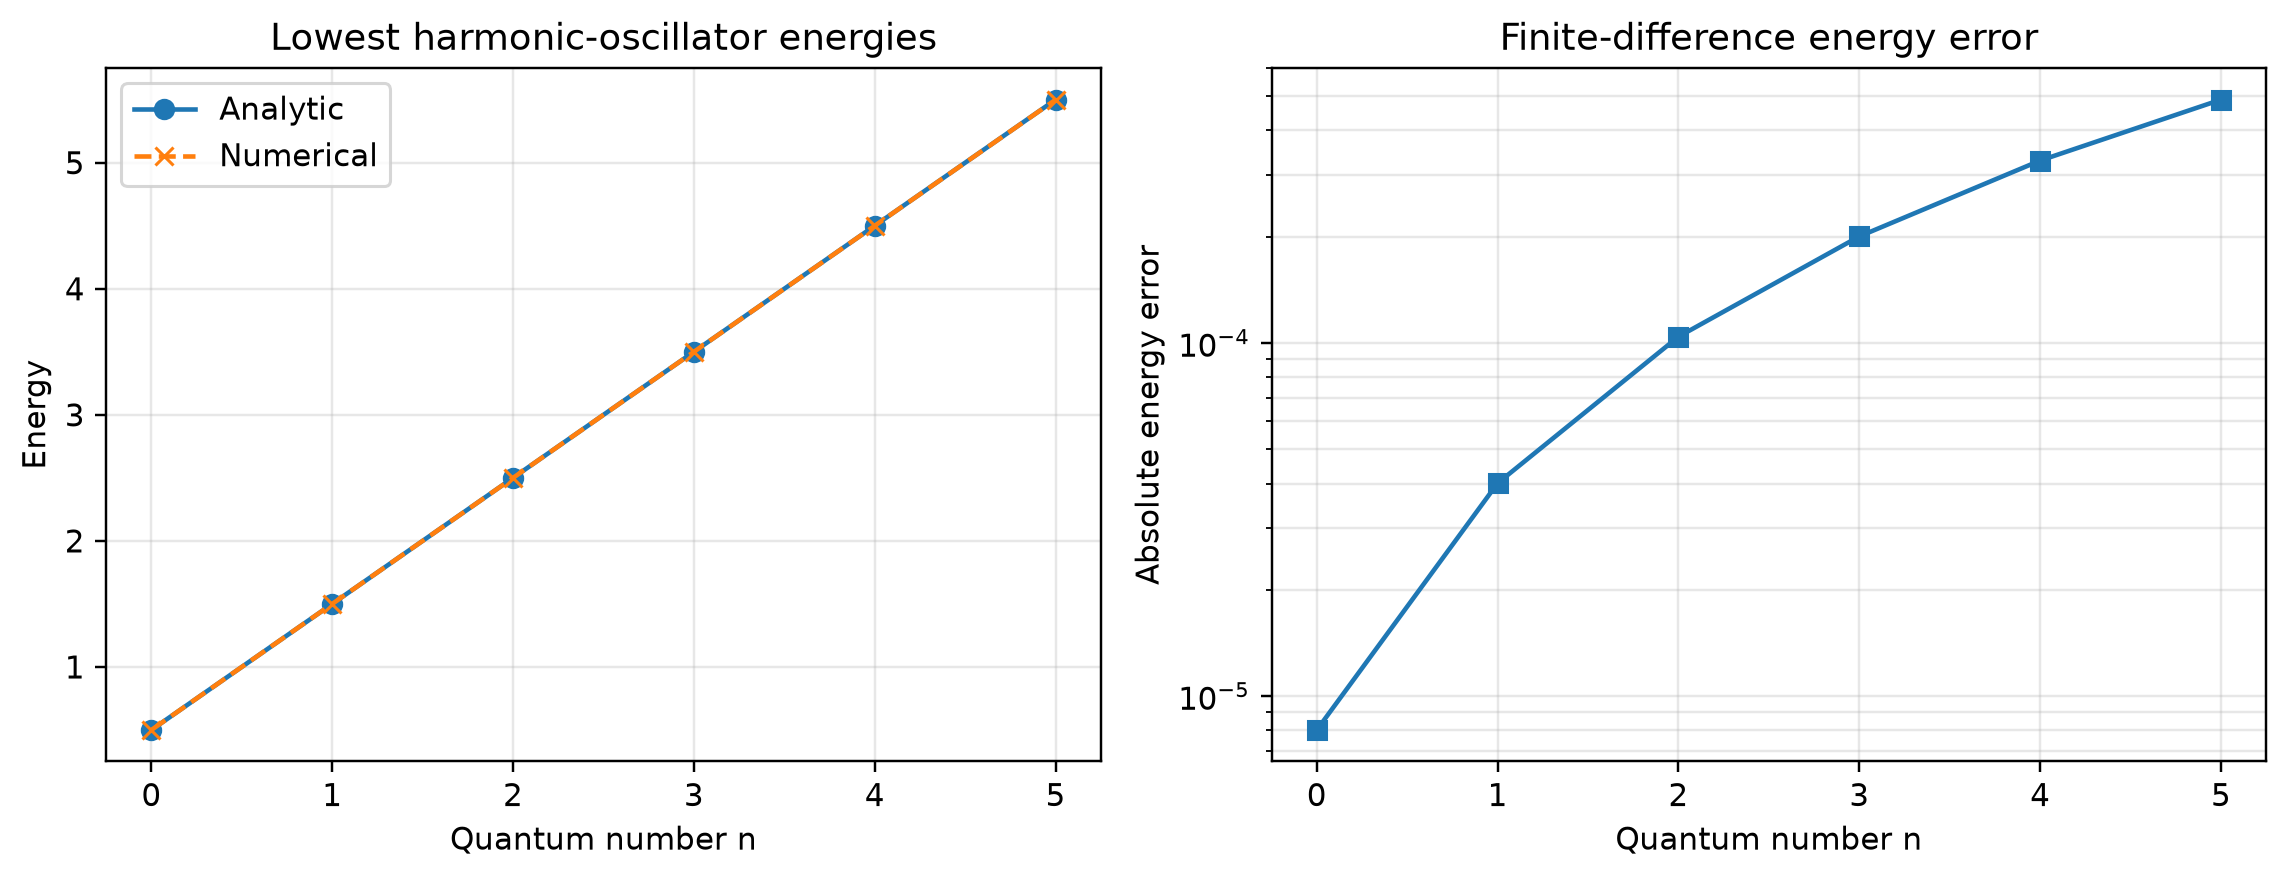
\includegraphics[width=0.88\textwidth]{energy_comparison.png}
\caption{The energies overlap visually (left), while the logarithmic
panel resolves the finite-difference error (right).}
\label{fig:energy}
\end{figure}

The two eigensolvers differ by at most \(3.92\times10^{-13}\), far below
the discretization error. The overlap matrix differs from the identity
by less than \(4.45\times10^{-16}\) in normalization and
\(2.76\times10^{-16}\) off diagonal. Before pointwise comparison, the
arbitrary sign of each numerical eigenvector is aligned with the analytic
state
\begin{equation}
 \psi_n(x)=
 \frac{H_n(x)e^{-x^2/2}}{\pi^{1/4}\sqrt{2^n n!}}.
\end{equation}
The largest wavefunction \(L^2\) error is \(2.52\times10^{-4}\), and the
largest probability-density \(L^1\) error is \(3.56\times10^{-4}\).
Every state has parity \((-1)^n\) and exactly \(n\) nodes. The largest
amplitude at the first interior point near a baseline boundary is
\(3.49\times10^{-11}\).

\clearpage
\section{Eigenstate Shapes}
Figure~\ref{fig:density} compares the numerical and analytic probability
densities. The curves overlap throughout the classically important
region. Higher states contain more nodes and extend farther from the
origin, explaining why their errors are larger on a fixed grid and why
they provide the stricter boundary test.

\begin{figure}[h]
\centering
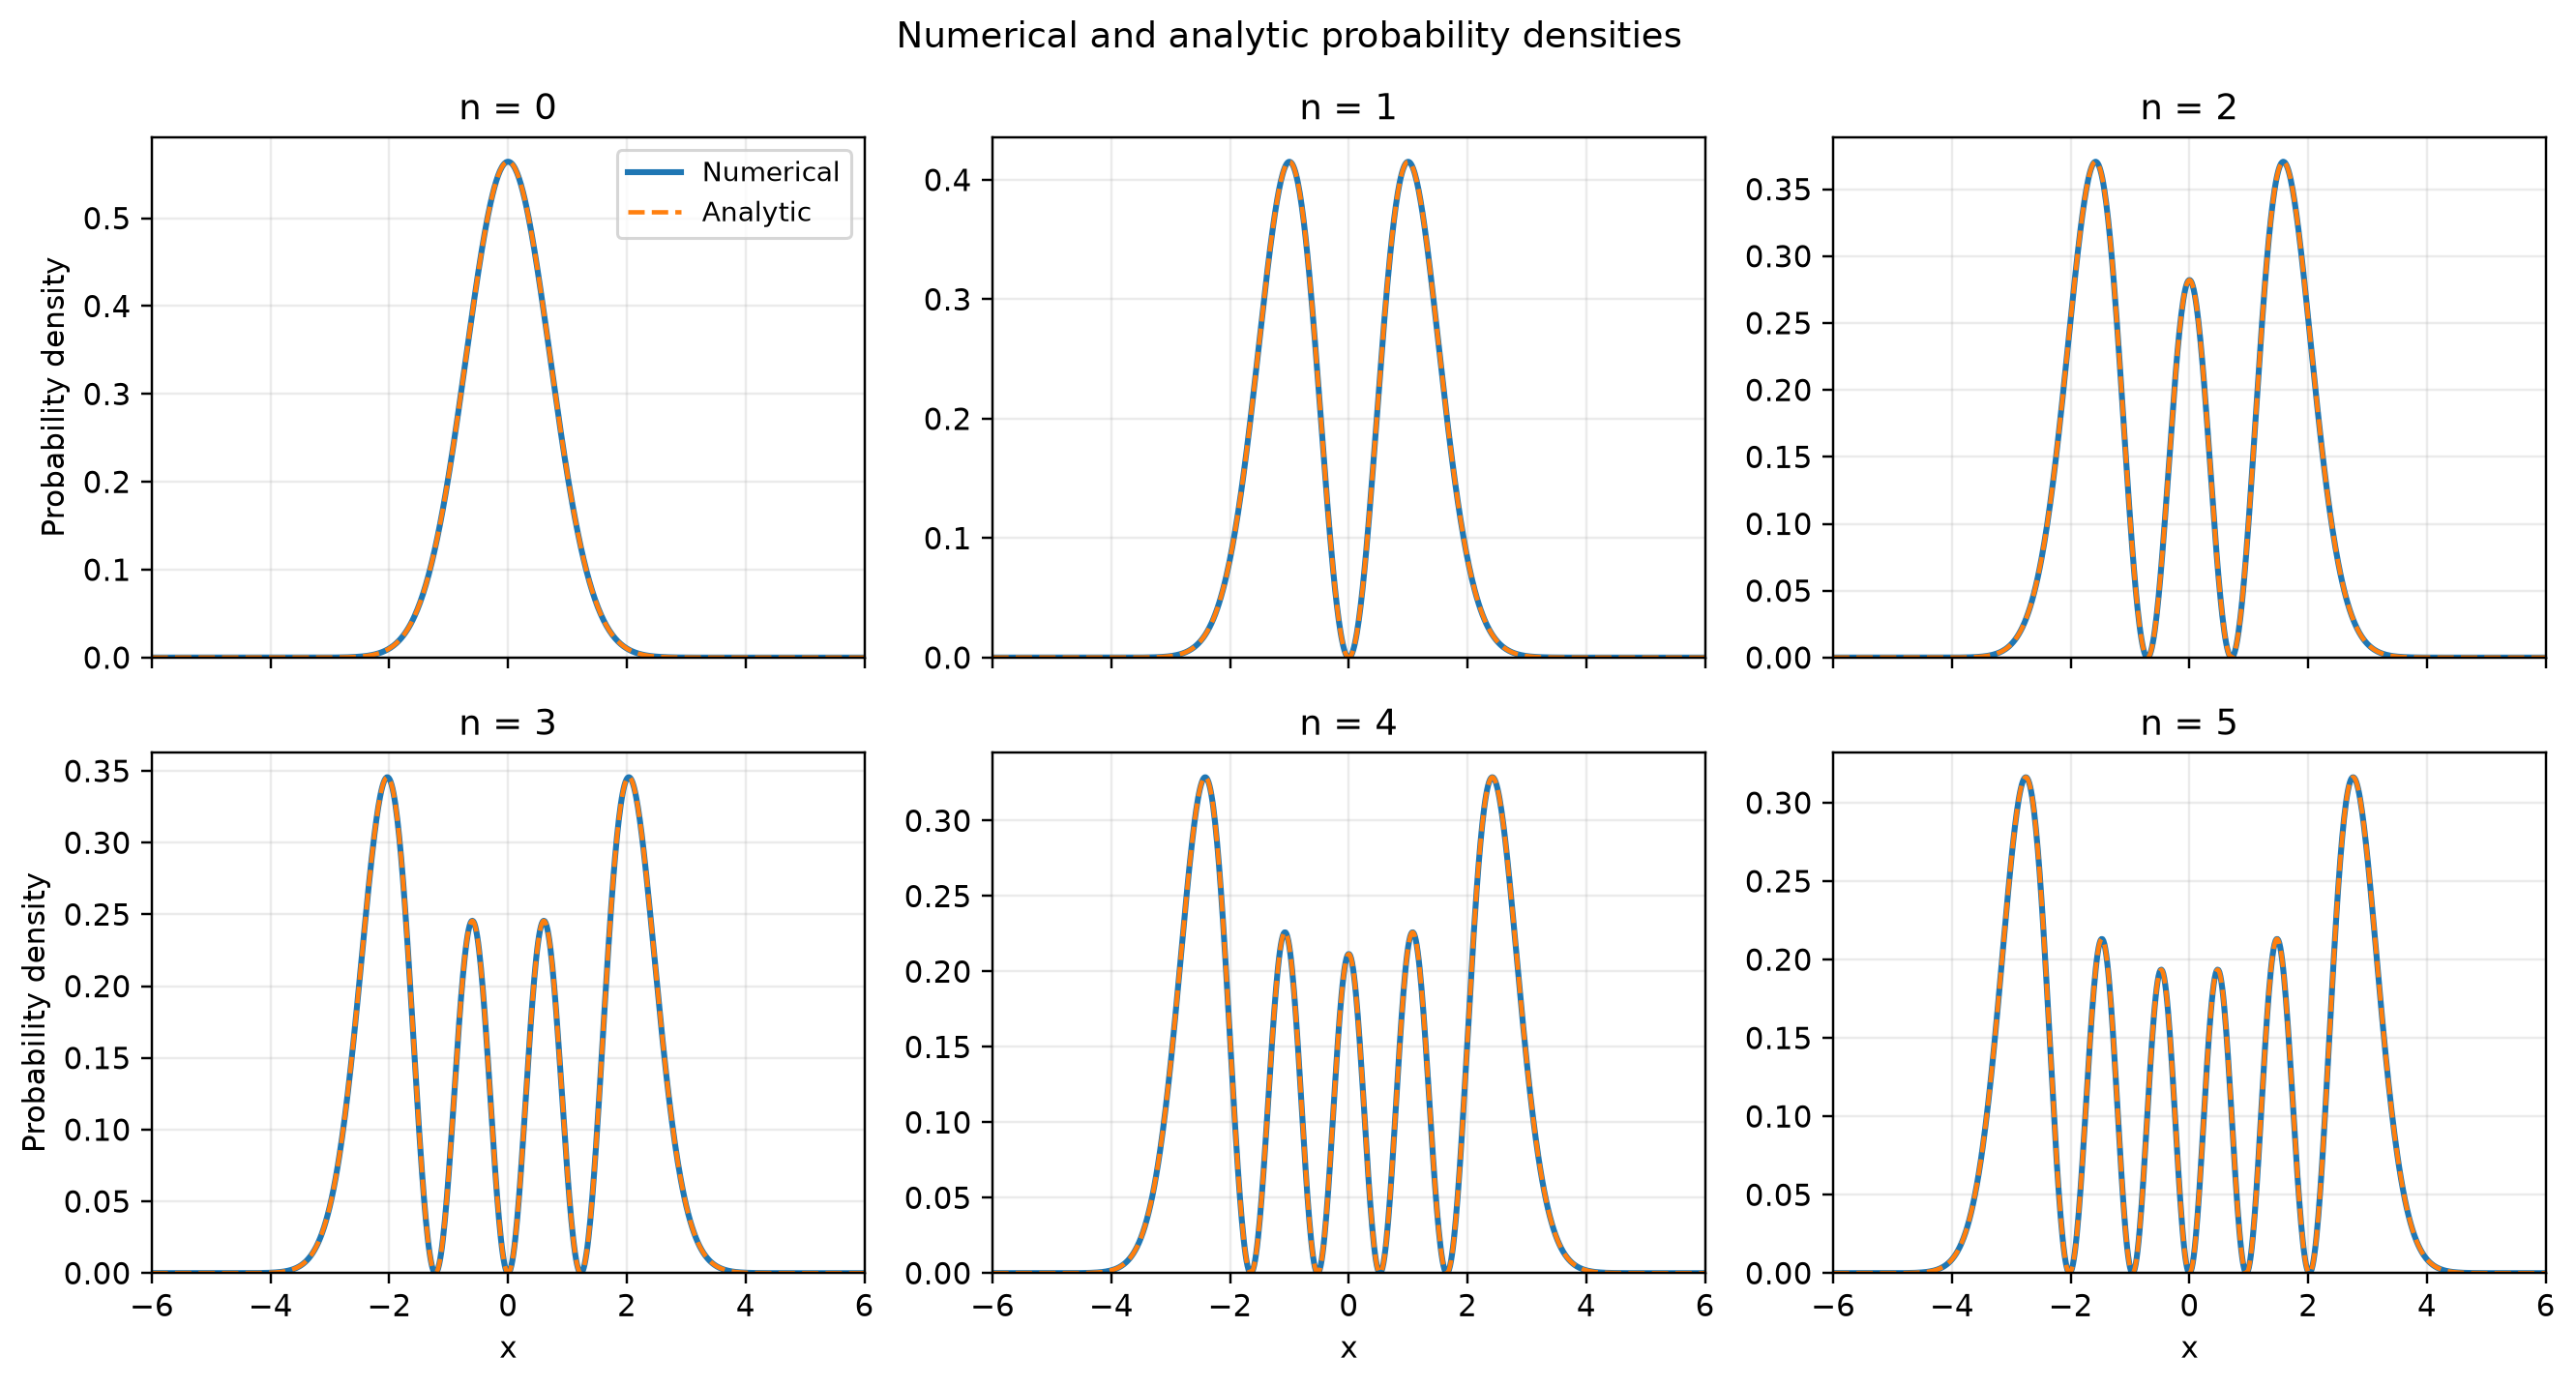
\includegraphics[width=0.93\textwidth]{probability_densities.png}
\caption{Numerical and analytic probability densities for the first six
states. Squaring removes the physically irrelevant global sign.}
\label{fig:density}
\end{figure}

\section{Separating the Two Numerical Errors}
Changing \(N\) and \(L\) simultaneously would mix discretization error
with boundary truncation. We therefore perform two independent studies.
For grid refinement, \(L=8\) is fixed while
\(N=200,400,800,1600,3200,6400\). Fitting
\(\log|\Delta E_n|\) against \(\log\Delta x\) gives orders from
\(2.0001\) to \(2.0005\), confirming the expected
\(O(\Delta x^2)\) behavior. Reducing the spacing by roughly a factor of
32 reduces every energy error by about \(10^3\).

For the box study, \(\Delta x=0.02\) is held fixed while \(L\) ranges
from 2.5 to 8 and \(N=\operatorname{round}(2L/\Delta x)+1\).
We monitor energy changes relative to \(L=8\) and the first-interior-point
amplitude. This is Anderson Mao's assigned convergence study.

\clearpage
\begin{figure}[t]
\centering
\begin{subfigure}[t]{0.43\textwidth}
 \centering
 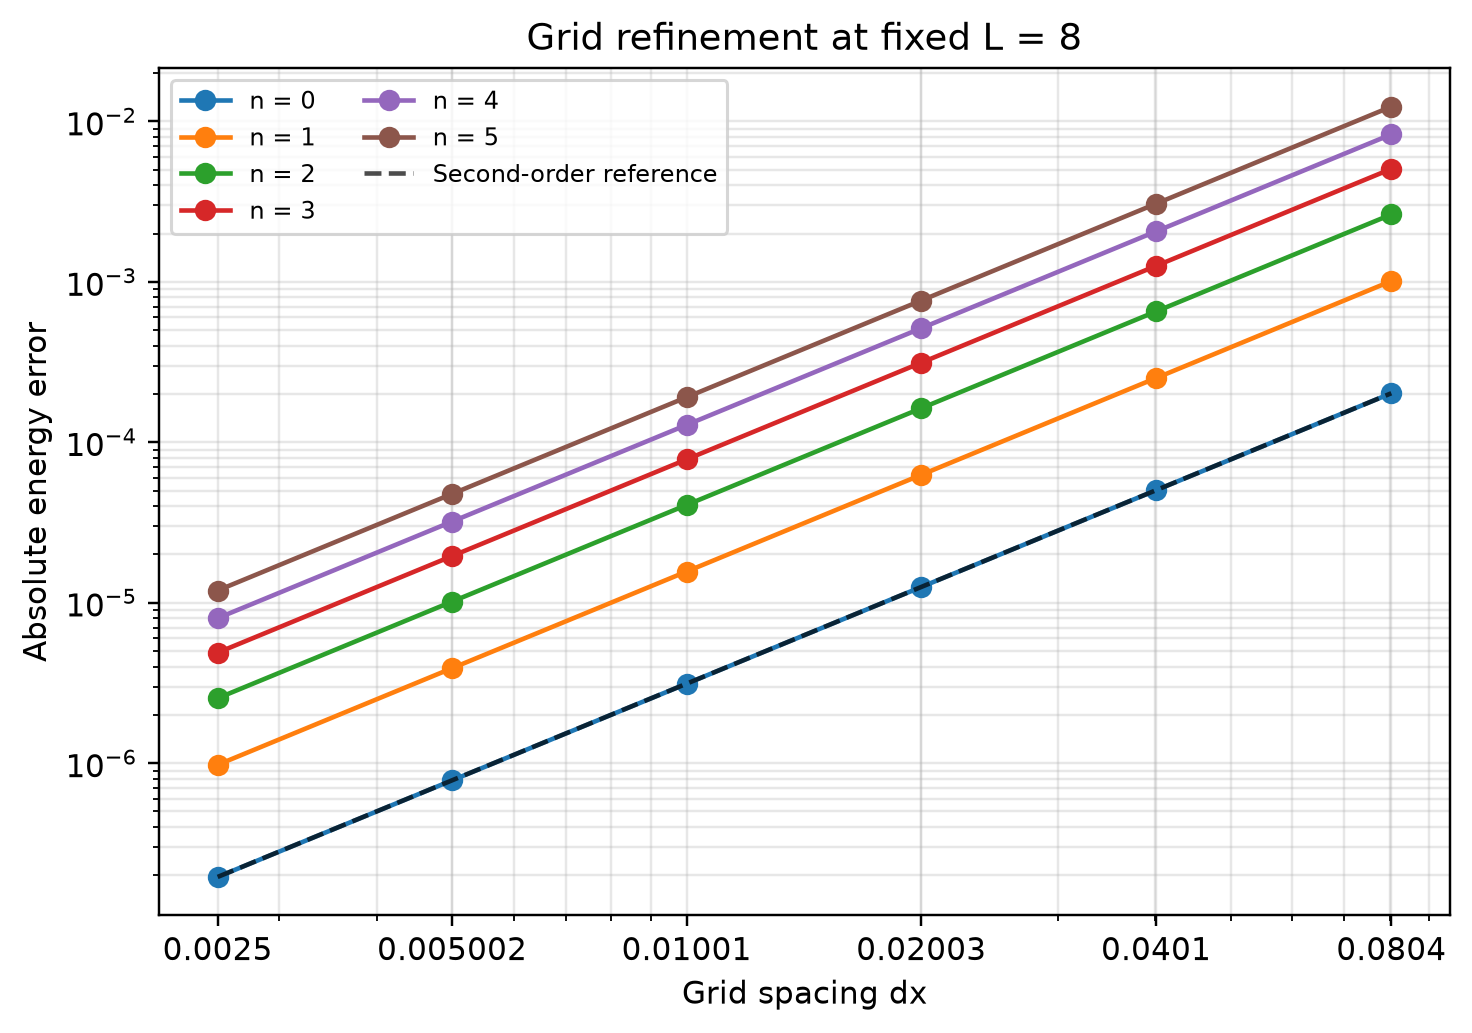
\includegraphics[width=\textwidth]{grid_convergence.png}
 \caption{Grid-spacing convergence at fixed \(L=8\).}
\end{subfigure}
\hfill
\begin{subfigure}[t]{0.55\textwidth}
 \centering
 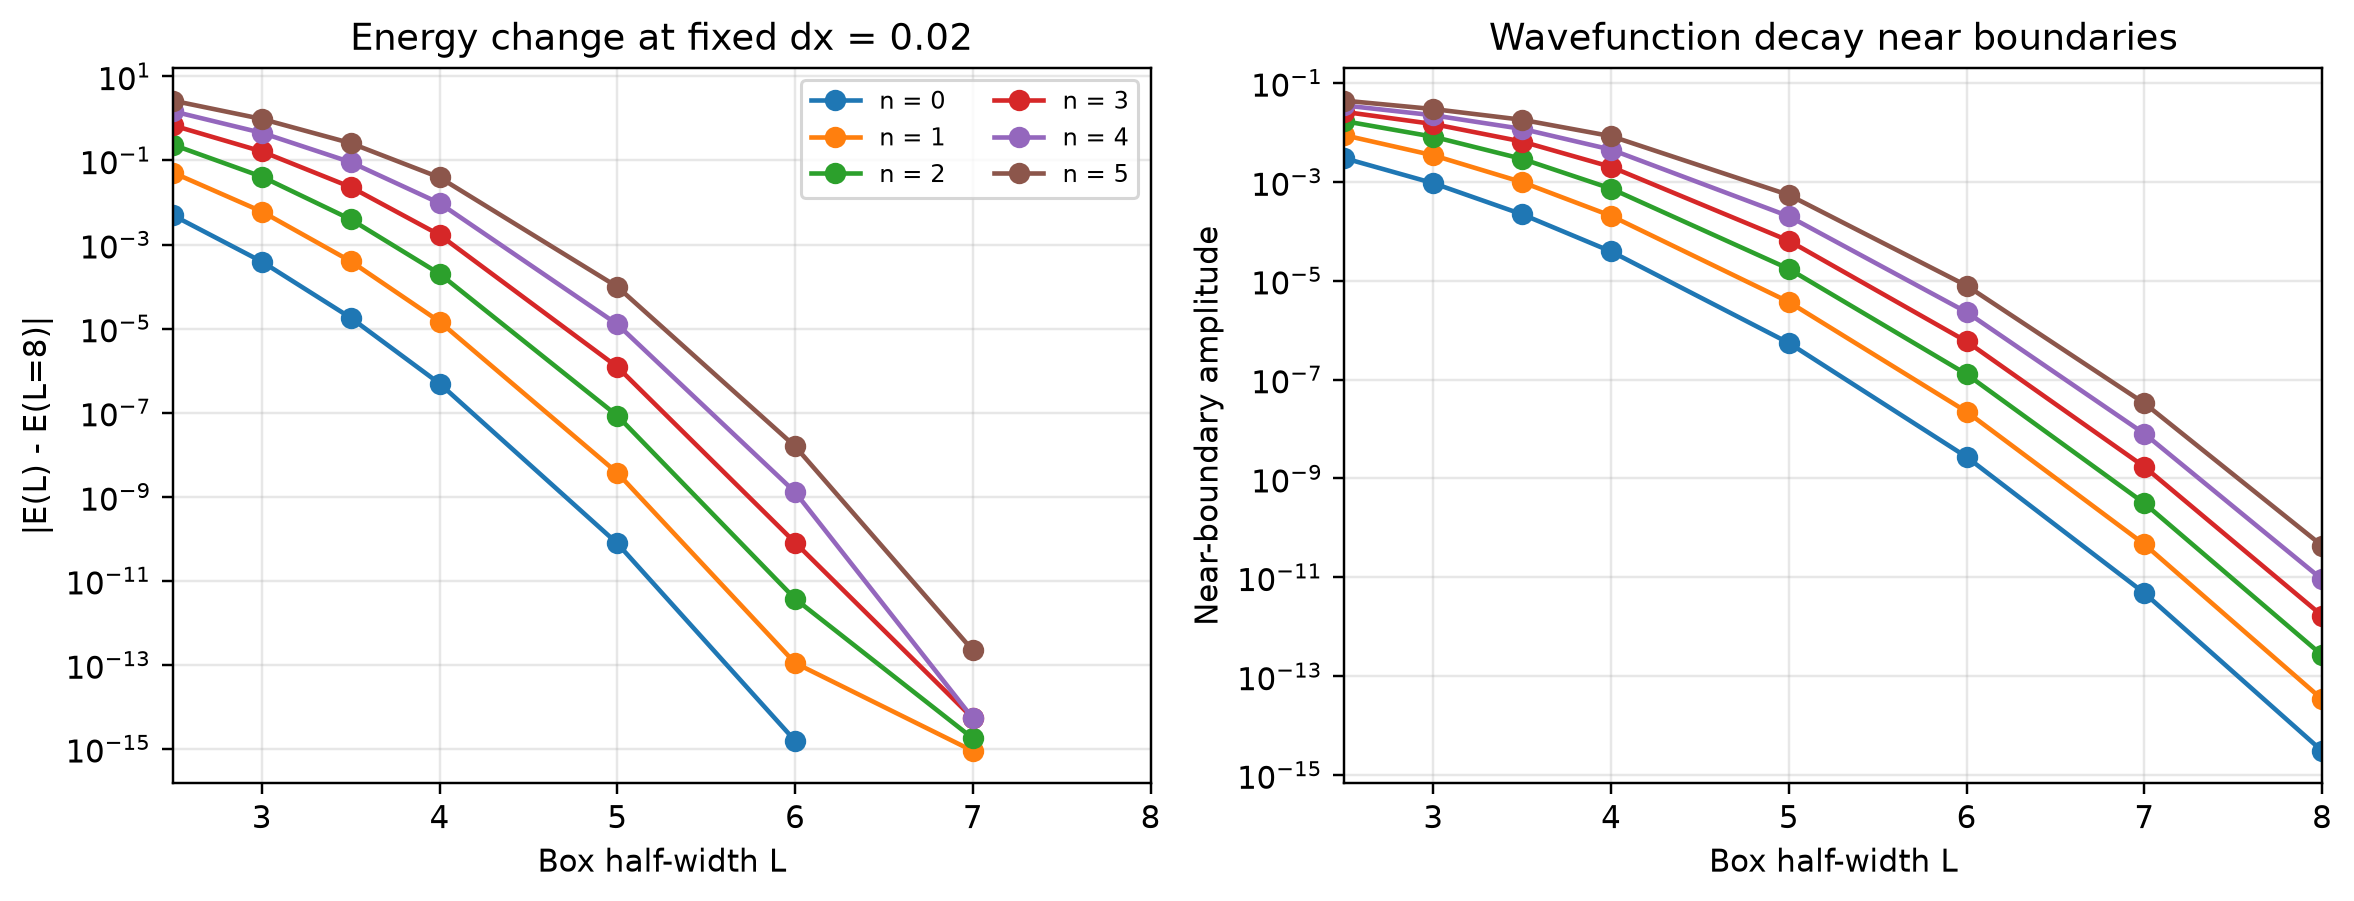
\includegraphics[width=\textwidth]{box_convergence.png}
 \caption{Box convergence at fixed \(\Delta x=0.02\).}
\end{subfigure}
\caption{The two numerical errors are varied independently.}
\label{fig:convergence}
\end{figure}

\begin{table}[h]
\centering
\small
\caption{Box-size convergence. The maxima are over states \(n=0,\ldots,5\).}
\label{tab:box}
\begin{tabular}{rrrr}
\toprule
\(L\) & \(N\) & \(\max_n|E_n(L)-E_n(8)|\) &
\(\max_n|\psi_n(x_{\mathrm{edge}})|\)\\
\midrule
2.5 & 251 & \(2.65\) & \(4.38\times10^{-2}\)\\
3.0 & 301 & \(9.72\times10^{-1}\) & \(2.96\times10^{-2}\)\\
4.0 & 401 & \(3.94\times10^{-2}\) & \(8.39\times10^{-3}\)\\
5.0 & 501 & \(9.87\times10^{-5}\) & \(5.42\times10^{-4}\)\\
6.0 & 601 & \(1.58\times10^{-8}\) & \(7.94\times10^{-6}\)\\
7.0 & 701 & \(2.19\times10^{-13}\) & \(3.33\times10^{-8}\)\\
8.0 & 801 & \(0\) & \(4.37\times10^{-11}\)\\
\bottomrule
\end{tabular}
\end{table}

Small boxes force the wider states to zero too early. For example,
\(E_5=8.15\) at \(L=2.5\), instead of 5.5. By \(L=7\), every energy is
stable relative to \(L=8\) at approximately \(10^{-13}\), and at
\(L=8\) all near-boundary amplitudes are below \(4.4\times10^{-11}\).
The nonzero energy-error plateau at large \(L\) is expected because
\(\Delta x\) is fixed; it is the discretization error measured by the
other study.

\clearpage
\section{Computational Cost}
The Hamiltonian is tridiagonal, so sparse storage grows linearly with the
number of interior points. Table~\ref{tab:cost} compares measured sparse
storage with the memory that a dense array would require. Timings vary by
computer, but the trend and memory advantage are clear. Vectorized array
operations are used throughout the production program; no Python loop is
needed to construct the Hamiltonian or calculate errors over the grid.

\begin{table}[h]
\centering
\small
\caption{Representative sparse-solver cost measurements for six states.}
\label{tab:cost}
\begin{tabular}{rrrrr}
\toprule
\(N\) & \(M\) & nonzeros & sparse MB (dense MB) & time (s)\\
\midrule
200  & 198  & 592   & 0.0079 (0.314) & 0.0014\\
800  & 798  & 2392  & 0.0319 (5.09)  & 0.0029\\
3200 & 3198 & 9592  & 0.1279 (81.8)  & 0.0066\\
6400 & 6398 & 19192 & 0.2559 (327.5) & 0.0112\\
\bottomrule
\end{tabular}
\end{table}

\section{Discussion and Conclusion}
The centered finite difference converts the differential equation into a
symmetric matrix eigenproblem whose numerical eigenstates pass independent
physical and algebraic checks. The computed energies lie slightly below
the exact values, as expected from the leading finite-difference error, and
the absolute errors increase with state number because higher states vary
more rapidly. Second-order grid convergence, stable large-box energies,
correct parity and nodes, boundary decay, and agreement between two
eigensolvers provide complementary evidence that the implementation is
correct.

The project delivers a reusable command-line program with a main function,
focused automated tests, CSV and JSON data, and publication-ready plots.
Possible extensions include a fourth-order stencil, a spectral basis, or
comparison with an anharmonic potential for which no elementary analytic
energy formula is available.

\section{Contributions and Reproducibility}
Brandon Blake developed the original Hamiltonian construction; Lizzie Kim
developed the initial plotting workflow; Keunmo Park developed the
eigensolver and analytic energy comparison; Ryan Dennis studied grid
convergence and computational cost; and Anderson Mao performed the
fixed-spacing box-size study and integrated the final reproducible program,
tests, results, and report. The group must add Marc's verified contribution
here before submission.

The repository README gives one-command usage instructions. Generative AI
was used to help integrate and document code, write automated checks, and
edit report prose. The group reviewed the generated material, ran the code,
and remains responsible for the numerical choices, interpretation, and
submitted work. External formulas and software interfaces were checked
against the sources below.

\begin{thebibliography}{9}
\small
\bibitem{mit13}
MIT OpenCourseWare, ``Lecture 13: Quantum Harmonic Oscillator,''
8.04 Quantum Physics I, Spring 2016.
\url{https://ocw.mit.edu/courses/8-04-quantum-physics-i-spring-2016/resources/lecture-13-quantum-harmonic-oscillator/}

\bibitem{mit1415}
MIT OpenCourseWare, ``Lectures 14--15: Quantum Harmonic Oscillator,
Creation and Annihilation Operators,'' 8.04 Quantum Physics I, Spring 2016.
\url{https://ocw.mit.edu/courses/8-04-quantum-physics-i-spring-2016/resources/lecture-14-15-quantum-harmonic-oscillator-creation-and-annihilation-operators/}

\bibitem{eigsh}
SciPy Developers, ``scipy.sparse.linalg.eigsh,'' SciPy API reference.
\url{https://docs.scipy.org/doc/scipy/reference/generated/scipy.sparse.linalg.eigsh.html}

\bibitem{tridiagonal}
SciPy Developers, ``scipy.linalg.eigh\_tridiagonal,'' SciPy API reference.
\url{https://docs.scipy.org/doc/scipy/reference/generated/scipy.linalg.eigh_tridiagonal.html}
\end{thebibliography}

\end{document}
